\documentclass[text05.tex]{subfiles}
\begin{document}
\subsection{デジタル入力\ruby{装置}{そう|ち}}
\subsubsection{ボタン}\label{button}
\begin{table}[H]
  \begin{widerrows}
    \begin{tabular}{|p{\colF}|p{\colG}|}	\hline
    \ruby{名称}{めい|しょう} & ボタン（ぼたん）\\ \hline
    \ruby{接続箇所}{せつ|ぞく|か|しょ} & デジタルコネクタ (3pin)\\ \hline
    \ruby{機能概要}{き|のう|がい|よう} & ボタンが\ruby{押}{お}されているか、\ruby{押}{お}されていないかを調べる\\ \hline
    \end{tabular}
  \end{widerrows} 
\end{table}

\begin{table}[H]
  \begin{widerrows}
    \begin{tabular}{|p{\colF}|p{\colG}|}	\hline
    サンプルコードの場所 & 05/digin.hsp\\ \hline
    raspiへの入力 & ボタンが\ruby{押}{お}されていると1、\ruby{押}{お}されていないと0の\ruby{値}{あたい}になる。\\ \hline
    raspiへの入力方法 & val = gpioin(GPIO番号)\\ \hline
    raspiからの出力 & なし\\ \hline
    raspiからの出力方法 & なし\\ \hline
    \end{tabular}
  \end{widerrows} 
\end{table}

\begin{table}[H]
  \begin{widerrows}
    \begin{tabular}{|p{\colF}|p{\colG}|} \hline
    使い道 & ゲームのコントローラーのボタン\\ \hline
    \ruby{注意事項}{ちゅう|い|じ|こう} & 強く\ruby{押}{お}して\ruby{壊}{こわ}さないように注意\\ \hline
    \ruby{補足}{ほ|そく} & ボタンを\ruby{押}{お}すことによって、中に入っている\ruby{金属}{きん|ぞく}が\ruby{繋}{つな}がり電気が流れます。\\ \hline
    \end{tabular}
  \end{widerrows} 
\end{table}

\begin{figure}[H]
  \begin{widerrows}
    \begin{tabular}{|p{\colH}|p{\colI}|p{\colH}|p{\colI}|} \hline
    外観 & 
    \begin{minipage}[t]{\linewidth}
      \smallskip
        \centering
        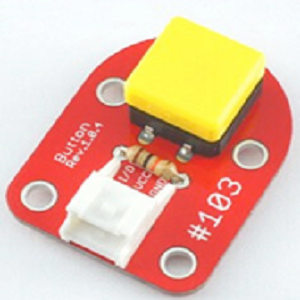
\includegraphics[width=0.5\linewidth]{../../asset/image/text05-img028.png}
        \caption{ボタン}
        \smallskip
      \end{minipage} &
      回路記号 & 
      \begin{minipage}[t]{\linewidth}
      \smallskip
        \centering
        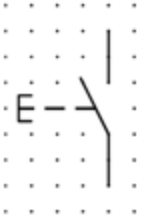
\includegraphics[width=0.3\linewidth]{../../asset/image/text05-img045.png}
        \caption{ボタンの回路図}
        \smallskip
      \end{minipage}\\ \hline
    \end{tabular}
  \end{widerrows} 
\end{figure}
\end{document}
